\documentclass[a4paper,man,natbib,floatsintext]{apa6}

\usepackage[english]{babel}
\usepackage[utf8x]{inputenc}
\usepackage[section]{placeins}
\usepackage{amsmath}
\usepackage{graphicx}
\usepackage{float}
\usepackage[colorinlistoftodos]{todonotes}
\usepackage{ragged2e}

\title{How Air Pollution Affects People's Daily Activities}
\shorttitle{How Air Pollution Affects People's Daily Activities}
\author{Chuanqi Jiang}
\affiliation{Tsinghua University}

\authornote{
Chuanqi Jiang, Department of Mathematics, Tsinghua University.\\
Chuanqi Jiang is now at Department of Mathematics, Tsinghua University.\\
This research was an assignment.\\
\noindent
Contact: jcq15@mails.tsinghua.edu.cn
}

\abstract{Abstract here}

\begin{document}
\renewcommand{\raggedright}{\leftskip=0pt \rightskip=0pt plus 0cm}
\maketitle

\section{Introduction}
Air pollution has been extensively studied in recent years. Many recent studies have focused on the impact of air pollution. Some researcher clearly shows that air pollution does harm to human health. Hazardous chemicals escape to the environment by a number of natural and/or anthropogenic activities, it has both acute and chronic effects on human health and affect a number of different systems and organs (Kampa \& Castanas, 2007). Air pollution causes many  respiratory diseases. Long-term exposure to combustion-related fine particulate air pollution is an important environmental risk factor for cardiopulmonary and lung cancer mortality (Pope et al., 2002). 

In order to deal with issues of why the air pollution makes so many effects on human health, a lot of researchers work on it and try to come up with the principles of pathogenicity. Many researchers have studied the principle of lung cancer caused by air pollution, and have got some results. Some ultra-fine particles, which size between $10^6nm/mL$, are able to provoke alveolar inflammation, with release of mediators capable, in susceptible individuals, of causing exacerbations of lung disease and of increasing blood coagulability (A. Seaton, D. Godden, W. MacNee, K. Donaldson, 1995). 

The results of these studies have made a great contribution to our understanding of air pollution and human health, they show the impact and the principles of pathogenicity for us. However, little work attempted to the impact of air pollution on people’s daily activities. We need to know how air pollution affects people's daily life. For example, how many people will give up outdoor activity if it is a polluted day? In this paper we give preliminary results for the impact. Specifically, we are going to talk about the difference of college students’ activity in Tsinghua University between clean air and polluted air. 


\section{Method}
\subsection{Questionnaire and participants}
We used questionnaire to survey the specific impact which air pollution caused to students in Tsinghua. The questionnare was devided into two parts: basic information and impact on daily activity and impact on mood. In the questionnare, question 1~6 were basic information about participants, question 7 were about daily activities. The second part was the most important part, we set six air pollution level by Air Quality Index (AQI). Participants were supposed to answer how high AQI would cause them stop the activity. In this way, we could know whether and how much the air pollution impact our daily activities. It was about these activities:

\begin{enumerate}
\item go to class in classroom
\item study at library
\item go to PE class
\item some relaxing outside sports (walk, ride .etc)
\item some intense sports (football, basketball .etc)
\item meet classmates outside
\item run outside
\item study in dormitory
\end{enumerate}

Although we wanted to work on all people around the world, however, limited by many factors, we could only do the survey in my school. So the participants of the study were \_ undergraduate students enrolled in Tsinghua University (notes: we don't know how many participants now). Participants are evenly distributed across the various faculties.

\subsection{Data processing}
For each activity, we knew the relation between AQI and the rate of student who wanted to do this activity, so we could use the Pearson product-moment correlation coefficient (PPMCC) to measure the relevance of the two variables. Then we did significant test to verification if the results are reasonable.
\newpage
\section{Results}
\subsection{The basic situation of the participants}

The first aim of this study was to show how air pollution affected people’s daily activities by talking about the difference of college students’ activity in Tsinghua University. First let's saw part one of the questionnare, which surveyed participants’ basic situation. The situation of participants was listed in Table 1. It could be seen that the number of people in various professions was even. Most of the participants were grade 1 or grade 2 (85.3\%). The next question was sports frequency. As shown in the questionnare, many people did sports once or twice a week (47.1\%), then 32.4\% people did sports three to five times a week. The data showed that the students had a moderate amount of exercise. As for wearing masks, nearly sixty percent of participants sometimes wear masks during polluted day, about twenty percent of people always wear masks. We could also know that 67.6\% participants had their own air purifiers in their dormitorys. According to the first part of questionnare, it was obvious that most people had the consciousness to protect themselves in polluted air.

\begin{table}
\centering
\caption{Participants.}
\begin{tabular}{c|c|c}
Major & No. of Participants & Percentage of All Participants\\\hline
Education & 10 & 29.4\% \\
Literature & 13 & 8.8\% \\
Science & 4 & 11.8\% \\
Engineering & 14 & 41.2\% \\
Medicine & 3 & 8.8\%

\end{tabular}
\end{table}

\subsection{The maximum AQI value that participants could accept}
The second part of the questionnaire was the core content of this survey. We have selected eight different activities. Participants were supposed to indicate the maximum AQI value that they could accept for participating in these activities. The range of options in the questionnaire was 0~200. It could be considered that the data satisfied the truncated normal distribution with an interval of [0,200]. For each activity, the maximum likelihood estimation was used to find the mean and variance of the corresponding normal distribution. The probability density function for the truncated normal distribution was
$$p(x) = \frac{
    \frac{1}{\sqrt{2\pi}\sigma} e^{-\frac{(x-a)^2}{2\sigma^2}}
}{
    \int_0^{200} \frac{1}{\sqrt{2\pi}\sigma} e^{-\frac{(t-a)^2}{2\sigma^2}} dt
}$$
and the likelihood function was
$$lik(a,\sigma) = \frac{
    \frac{1}{(2\pi)^{\frac{n}{2}}\sigma ^n} e^{-\frac{1}{2\sigma^2}\sum_{i=1}^n(x_i-a)^2}
}{
    (\int_0^{200} \frac{1}{\sqrt{2\pi}\sigma} e^{-\frac{(t-a)^2}{2\sigma^2}} dt)^n
}$$
where $x_i, 1\leq i\leq n$ mean the data we got from questionnares.

The figure of the likelihood function was drawn in Matlab. We could find the initial point, which was used to calculate the maximun of the likelihood function, from the figure. And then the minimum point of the likelihood function was obtained by the Newton method. Taking the event "into the classroom" as an example, the image of the likelihood function was shown in Fig. 1. Select the initial point $(40,100)$, we could find the minimum point $(36.9,89.0)$. In other words, the mean value of the highest AQI that participants could accept in the classroom was $89.0$ , and the variance was $36.9$.

\begin{figure}
\centering
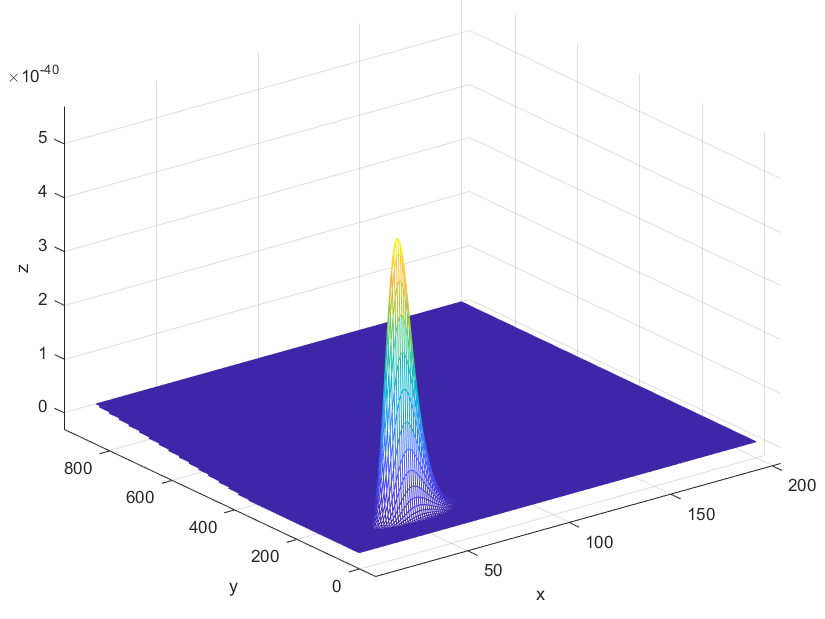
\includegraphics[width=0.8\textwidth]{1.png}
\caption{\label{fig:frog}Likelihood function about event "into the classroom".}
\end{figure}

The above operations were performed on all eight activities and the average and variance of the highest AQI values that the participants were able to accept under different activities were shown in Table 2. From Table 2 we could see that study in dormitory could accept the highest level of air pollution (115.5). On the contrary, some intense sports were most sensitive to air quality (72.7). Contrasting between the eight activities, the highest acceptable AQI for each activity was distributed around 100. The variances were distributed in range 30~50, so participants had about the same degree of dispersion of AQIs for the eight activities.

\begin{table}
\centering
\caption{The highest AQI values that the participants were able to accept under different activities.}
\begin{tabular}{c|c|c}
Activity & mean AQI & variance \\
\hline
go to class in classroom & 89.0 & 36.9 \\
study at library & 98.8 & 47.1 \\
go to PE class & 95.8 & 39 \\
some relaxing outside sports (walk, ride .etc) & 88.3 & 34.4 \\
some intense sports (football, basketball .etc) & 72.7 & 42.6 \\
meet classmates outside & 85.6 & 44.1 \\
run outside & 84.3 & 48.1 \\
study in dormitory & 115.5 & 45.8

\end{tabular}
\end{table}

\section{Discussion}

In this study, we studied the highest AQI value that everyone could accept under the eight activities. According to life experience, the amount of exercise capacity in the dormitory is small, so it should be the highest acceptable AQI value. Seeing the result, we found that the mean value of the study in dormitory was really the highest. Also, the low highest acceptable AQI value suggests that, the same to the hypothesis, it has great difference of college students’ activity between clean air and polluted air. This conclusion is most obvious for intense outdoor sports. Similar to other studies done before, this study illustrates the negative effects of air pollution from another perspective.

If people's highest accepted AQI meets the normal distribution in results part, then the percentage of people participating in the corresponding activities under different AQIs can be calculated, it is shown in Table 3. Pope (2002) suggested that Long-term exposure to combustion-related fine particulate air pollution is an important environmental risk factor for cardiopulmonary and lung cancer mortality. This has provided a theoretical basis for people to go out less in the polluted air.

\begin{table}
\centering
\caption{The percentage of people participating in the corresponding activities under different AQIs.}
\begin{tabular}{c|c|c|c|c|c|c|c|c}
AQI & class & lib & PE & sports(relax) & sports(intense) & meet & run & dormitory \\
\hline
20 & 0.969 & 0.953 & 0.974 & 0.976 & 0.892 & 0.932 & 0.909 & 0.981 \\
40 & 0.908 & 0.894 & 0.924 & 0.920 & 0.779 & 0.849 & 0.821 & 0.950 \\
60 & 0.784 & 0.795 & 0.821 & 0.795 & 0.617 & 0.719 & 0.693 & 0.887 \\
80&0.596 & 0.655 & 0.657 & 0.595 & 0.432 & 0.551 & 0.536 & 0.781 \\
100&0.383 & 0.490 & 0.457 & 0.367 & 0.261 & 0.372 & 0.372 & 0.632 \\
120&0.200 & 0.326 & 0.267 & 0.178 & 0.133 & 0.218 & 0.229 & 0.461 \\
140&0.083 & 0.191 & 0.129 & 0.066 & 0.057 & 0.109 & 0.123 & 0.296 \\
160&0.027 & 0.097 & 0.050 & 0.019 & 0.020 & 0.046 & 0.058 & 0.166 \\
180&0.007 & 0.042 & 0.015 & 0.004 & 0.006 & 0.016 & 0.023 & 0.080

\end{tabular}
\end{table}


We intend to further study how to take measures to reduce the impact of air pollution on people's activities and how to quantify the effectiveness of these measures. For example, change outdoor sports to indoor sports or install an air purifier. We hope that the follow-up study will help people reduce the impact of air pollution.


\newpage
\section{References}


\footnotesize{

\noindent
\hangafter=1
\setlength{\hangindent}{4em}
Pope III CA, Burnett RT, Thun MJ, et al. Lung Cancer, Cardiopulmonary Mortality, and Long-term Exposure to Fine Particulate Air Pollution. JAMA. 2002;287(9):1132-1141. 

\noindent
\hangafter=1
\setlength{\hangindent}{4em}
A. Seaton, D. Godden, W. MacNee, K. Donaldson, Particulate air pollution and acute health effects. The Lancet. 1995;345(8943):176-178.

\noindent
\hangafter=1
\setlength{\hangindent}{4em}
Marilena Kampa, Elias Castanas, Human health effects of air pollution. Elsevier. 2008;151(2):362-367.

}


% You can add inline TODO comments with the todonotes package, like this:
% \todo[inline, color=green!40]{This is an inline comment.}

%Use the table and tabular commands for basic tables --- see Table~\ref{tab:widgets}, for example. You can upload a figure (JPEG, PNG or PDF) using the files menu. To include it in your document, use the includegraphics command as in the code for Figure~\ref{fig:frog} below.

% Commands to include a figure:
%\begin{figure}
%\centering
%\includegraphics[width=0.5\textwidth]{frog.jpg}
%\caption{\label{fig:frog}This is a figure caption.}
%\end{figure}



%You can make lists with automatic numbering \dots

% \begin{enumerate}
% \item Like this,
% \item and like this.
% \end{enumerate}
% \dots or bullet points \dots
% \begin{itemize}
% \item Like this,
% \item and like this.
% \end{itemize}


%\bibliography{example}

\end{document}

%
% Please see the package documentation for more information
% on the APA6 document class:
%
% http://www.ctan.org/pkg/apa6
%